\documentclass[12pt,final,fleqn]{article}

% basic packages
\usepackage[margin=1in] { geometry }
\usepackage{amssymb,amsmath, bm}
\usepackage{verbatim}
\usepackage[latin1]{inputenc}
%\usepackage[OT1]{fontenc}
\usepackage{setspace}
\usepackage{enumitem}
\usepackage{url}
\usepackage[font={bf}]{caption}
\usepackage{float}
%\usepackage{pgfplots}
%\usepackage[font={bf}]{caption}
\usepackage{setspace}
\usepackage{latexsym}
%\usepackage{euscript}
\usepackage{graphicx}
\usepackage{marvosym}
\usepackage{amsmath} 
\usepackage{authblk}
\usepackage{xcolor}
%\usepackage[varg]{txfonts}  Older version of ``g'' in math.

% bibliography packages
\usepackage[natbibapa]{apacite}
\bibliographystyle{apacite}
\bibpunct{(}{)}{;}{a}{}{,}
\renewcommand{\bibname}{References}

% hyperref options
\usepackage{color}
\usepackage{hyperref}
\usepackage{xcolor}
\hypersetup{
    colorlinks,
    linkcolor={blue!50!black},
    citecolor={blue!50!black},
    urlcolor={blue!80!black}
}
\newcommand*{\Appendixautorefname}{Appendix}
\renewcommand*{\sectionautorefname}{Section}
\renewcommand*{\subsectionautorefname}{Section}
\newcommand{\aref}[1]{\hyperref[#1]{Appendix~\ref{#1}}}

% packages for tables
\usepackage{longtable}
\usepackage{booktabs, threeparttable}
\usepackage{threeparttablex}
%\usepackage{tabularx}
% dcolumn package
\usepackage{dcolumn}
\newcolumntype{.}{D{.}{.}{-1}}
\newcolumntype{d}[1]{D{.}{.}{#1}}
\captionsetup{belowskip=10pt,aboveskip=-5pt}
\usepackage{multirow}
% rotating package
\usepackage[figuresright]{rotating}
\usepackage{pdflscape}
\usepackage{subcaption}

% packages for figures
\usepackage{grffile}
\usepackage{afterpage}
\usepackage{float}
\usepackage[section]{placeins}


% theorem package
\usepackage{theorem}
\theoremstyle{plain}
\theoremheaderfont{\scshape}
\newtheorem{hyp}{Hypothesis}
\newtheorem{theorem}{Theorem}
\newtheorem{algorithm}{Algorithm}
\newtheorem{assumption}{Assumption}
\newtheorem{lemma}{Lemma}
\newtheorem{proposition}{Proposition}
\newtheorem{remark}{Remark}
\newcommand{\qed}{\hfill \ensuremath{\Box}}
\newcommand\indep{\protect\mathpalette{\protect\independenT}{\perp}}
\DeclareMathOperator{\sgn}{sgn}
\DeclareMathOperator{\tr}{tr}
\DeclareMathOperator{\argmin}{arg\min}
\DeclareMathOperator{\argmax}{arg\max}
\def\independenT#1#2{\mathrel{\rlap{$#1#2$}\mkern2mu{#1#2}}}
\providecommand{\norm}[1]{\lVert#1\rVert}
\renewcommand\r{\right}
\renewcommand\l{\left}
\newcommand\E{\mathbb{E}}
\newcommand\dist{\buildrel\rm d\over\sim}
\newcommand\iid{\stackrel{\rm i.i.d.}{\sim}}
\newcommand\ind{\stackrel{\rm indep.}{\sim}}
\newcommand\cov{{\rm Cov}}
\newcommand\var{{\rm Var}}
\newcommand\SD{{\rm SD}}
\newcommand\bone{\mathbf{1}}
\newcommand\bzero{\mathbf{0}}

% dotted lines in tables
%\usepackage{arydshln}

\usepackage{pdflscape}

% spacing between sections and subsections
\usepackage[compact]{titlesec}

% times new roman
%\usepackage{times}

% appendix settings
\usepackage[toc,page,header]{appendix}
\renewcommand{\appendixpagename}{\centering Appendices}
\usepackage{chngcntr}
\usepackage{etoolbox}
\usepackage{lipsum}


% file paths and definitions
\makeatletter
\newcommand*\ExpandableInput[1]{\@@input#1 }
\makeatother

\setlength{\mathindent}{1cm}
\allowdisplaybreaks[4]
\doublespacing
%\special{pdf: pagesize width 8.5truein height 11.0truein}

\titleformat{\subsection}
  {\itshape\large}{\thesubsection}{1em}{}

\setcounter{tocdepth}{1}

%--------------------------------------------------------------------------------------
% BEGIN DOCUMENT
%--------------------------------------------------------------------------------------

\begin{document}
\singlespace
\title{\textbf{Legislators and use of evidence: double standards? A field experiment \\
(Pre-Analysis Plan)}\vspace{-1ex}\thanks{}}
% Thanks
\author{Ang�le Delevoye\thanks{angele.delevoye@yale.edu}\vspace{-1ex}}
\author{Trevor Incerti\thanks{trevor.incerti@yale.edu}\vspace{-1ex}}
\affil{\textit{Yale University}\vspace{-2.5ex}}
\date{\today}
\maketitle

\begin{abstract}
\noindent
The bipartisan Foundations for Evidence-Based Policymaking Act of 2018 stresses the need for evidence-based policy-making. We propose a field experiment that tests whether legislators are actually more receptive to higher standards of research evidence when receiving and evaluating policy information. A related question is if legislators possess sufficient knowledge of evidence standards to be able to differentiate between varying standards of research quality. This pre-analysis plan proposes a field-experimental research design dedicated to answering these questions, and pre-registers the procedures that will be used to conduct the analysis.
\end{abstract}

\pagebreak

\doublespace

\begin{center}
%[PREMIMINARY DRAFT: INCOMPLETE]
\end{center}

\section{Introduction} \label{sec:Introduction}

The need for more evidence-based policy-making is the object of a rare bipartisan agreement. Congress passed the Foundations for Evidence-Based Policymaking Act in 2018 - legislation sponsored by then-House Speaker Paul Ryan (R-WI) and Senator Patty Murray (D-WA). Only 17 representatives voted against, and it passed the Senate by unanimous consent. Policy-makers' intentions are clear, but do their behaviors and knowledge align with those intentions? Are policy-makers really more receptive to higher standards of evidence when evaluating policy-information? Moreover, even if policymakers want to adopt policies based on high-quality evidence, do they have sufficient knowledge of evidence standards to be able to differentiate between research of varying quality? 

We propose a field experiment to test: (1) whether policymakers give more credence to high quality research, and (2) if policymakers can recognize differences in research quality. Our research design would entail contacting policy-makers with information regarding research on a potential educational policy while randomizing the kind of research design from which study derives its evidence - from a simple regression to a well-conducted RCT. We would also randomize whether we provide the policy-maker with information about varying standards of evidence within academic research (e.g. informing them that an RCT is considered the gold standard in causal inference and policy evaluation studies). 

Our pre-analysis first presents the theory and existing literature we hope to advance. In particular, we hope to build on existing experimental studies that have contacted American policy-makers. Next, we present the details of our proposed experimental design: treatment (choice of policy and evidence standard), logistics (partnership with a 3rd party organization), outcome measures, and ethical considerations. These details on the design are still preliminary, and several open questions remain. We conclude with a power analysis for the proposed experiment.


\section{Theory} \label{sec:Theory}
\subsection{Evidence in policymaking}  \label{sec: evidence}

A growing literature examines if, when, and how evidence and expertise is used in policy-making. The conventional wisdom from the this literature in the US Congressional context has long been that evidence and information do not matter. Legislators are focused on reelection \citep{mayhew1974congress}, power within Congress \citep{fenno1973congressmen}, and responding to pressures from local constituents \citep{fenno2002home}. \citet{schick1976supply} concluded in 1976 that ``Congress is not a natural habit for policy analysis," and \citet{lindblom2018science} states that the best Congress can do is ``muddle through" given institutional constraints and lack of time and resources. 

Recently, however, scholars have called for a more nuanced understanding of the use of evidence in policy-making \citep{patashnik2016can}, despite well-identified methodological challenges \citep{mandell1984approaches}. Case studies have suggested that evidence is used in policy-making, but we need a better understanding of how (much), when and why. Scholars have also examined the supply of scientific evidence, and have looked how scientists can maximize the use of scientific evidence. \citet{cairney2016politics} lays out two types of shortcuts used by legislators, rational decision-making and irrational decision-making drawing on emotions, beliefs and habits. He argues that scientists have mostly focused on the former, and that they should do a better job at accompanying evidence with simple stories to exploit the emotional or ideological biases of policymakers. We hope to test and measure legislators' ability to respond to the first, rational type of stimulus. 

Experimental research on messenger effects (i.e. does the source of information matter?) may also be relevant to our research design. Source credibility theory hypothesizes that high-credibility sources are more effective in matters of persuasion than low-credibility sources and distinguishes between expertise and trustworthiness as sources of credibility \citep{pornpitakpan2004persuasiveness}. Additional research has found that trustworthiness (i.e. being ``liked'') is more effective than expertise (i.e. being ``right'') \citep{mcginnies1980better}, implying that the source of evidence is important in addition to evidence quality. This implies that the institution responsible for the research may be highly important, and should therefore be held constant across treatment groups and should be a trusted, non-partisan instituion. 

Our initial goal is to conduct this experiment with the U.S. Congress, however it may be necessary to change our focus to the the state or local level for power or logistical reasons. In this case, we would need to consider literature on policy deliberation in state and local politics. 

Finally, this project may speak to broader theoretical questions on the functioning of our current democracies, and the potential gaps between reality and the ideals of deliberative democracies. In this sense, we hope this project will contribute to ongoing discussions within philosophy of science, such as perceptions of research methods and consumption of scientific evidence outside of the academy.

\subsection{Legislator contact experiments}  \label{sec: contact experiments}

Randomized contact of legislators in American politics research remains relatively rare. \autoref{tab:audit_experiments} below summarizes previous field-experimental studies that have contacted legislators. Our design most closely resembles a mix of the experiments conducted by \citet{butler2011politicians} and \citet{kalla2016campaign}. Our factorial design will come close to \citet{butler2011politicians}'s 2x3 design (and may use their contact list for state legislatures). We also plan to emulate \citet{kalla2016campaign}'s use of a third party organization to contact legislators, as well as their more nuanced outcome measure: both rate of response to emails and the seniority of the person who has agreed to meet with the organization. The use of roll call votes as in \citet{bergan2009does} is likely only possible for an experiment that targets one bill in one Chamber. 

%Roll call votes are not a realistic outcome measure in our case: even if we were to reach out with policy information on a specific bill, too much would happen between us reaching out and the MC eventual vote for us to be able to isolate the effect of us reaching out. [That should be ok? The treatment would still delivered randomly.]




\begin{sidewaystable}[]
\caption{Audit experiments conducted with U.S. policy-makers}
\label{tab:audit_experiments} 
\bigbreak
\tiny
\begin{tabular}{|l|l|l|l|l|l|l|l|l|}
\hline
Reference      
& Federal/State                                                                                                                        & Arms 
& Treatment                                                                                                           
& Design                                                                                                                                                        & Outcome 
& 3rd party?                                                                                                                                                                                                                                                  \\ \hline
 \citet{bergan2009does}        
& \begin{tabular}[c]{@{}l@{}}State \\ (New Hampshire) \end{tabular}                                                  & 1
& \begin{tabular}[c]{@{}l@{}} Contacted \\ by activists \end{tabular}                                           & \begin{tabular}[c]{@{}l@{}}Matched pairs \\ (multimembers districts)\\ Randomization within party\\ and district stratas\end{tabular}                         
& Roll Call votes                                                                                            
& \begin{tabular}[c]{@{}l@{}}Yes: coalition of \\ public health-related groups\\  organizing a grassroots email \\ lobbying campaign by activists\end{tabular}                                                                                              
  \\ \hline
 \citet{butler2011politicians}       & \begin{tabular}[c]{@{}l@{}}4,859 state legislators\\ (44 states)\end{tabular}                                                        & 2x3          & \begin{tabular}[c]{@{}l@{}}Black or \\ white name and\\ party (D/R/blank)\\ of email sender\end{tabular}            & \begin{tabular}[c]{@{}l@{}}Block randomization\\ by state, chamber, \\ party, and whether\\ legislator is up for \\ reelection\end{tabular}                   & \begin{tabular}[c]{@{}l@{}}Rate of response\\ to emails\end{tabular}                                       & No                                                                                                                                                                                                                                                          \\ \hline
 \citet{kalla2016campaign}     & \begin{tabular}[c]{@{}l@{}}US Congress \\ 191 offices that had \\ not yet sponsored bill \end{tabular} & 1            & \begin{tabular}[c]{@{}l@{}}Reveal in email that\\ prospective attendees had\\ contributed to campaigns\end{tabular} & \begin{tabular}[c]{@{}l@{}}Blocks of 3 offices: closest\\ similarity on multiple \\ covariates\\ 1 treated, 2 control in each\\ of the 64 blocks\end{tabular} & \begin{tabular}[c]{@{}l@{}}Rate of response\\ to emails and\\ seniority of proposed\\ meeting\end{tabular} & \begin{tabular}[c]{@{}l@{}}Yes: liberal political organization \\ trying to set meetings between offices\\ and constituents who had previously \\ given to campaigns. \\ Goal of the meetings: rally support for \\ a bill banning a chemical.\end{tabular} 
 \\ \hline
  \citet{doberstein2017whom}     & \begin{tabular}[c]{@{}l@{}}1,108 \\ Canadian bureaucrats\end{tabular} & 2x2           & \begin{tabular}[c]{@{}l@{}}Source of the\\ policy information \\(academic, think tanks, \\ research-based \\advocacy groups) \end{tabular} & \begin{tabular}[c]{@{}l@{}}Sources in \\treatment groups \\ were falsified \\  Pre treatment survey\\ for covariates \end{tabular} & \begin{tabular}[c]{@{}l@{}} Credibility assessment of \\each of 5 research articles \\ Based on summaries \\ And ranking of the 5 articles \end{tabular} & \begin{tabular}[c]{@{}l@{}}No.\end{tabular} 
   \\ \hline
  \citet{zelizer2018responsive}     & \begin{tabular}[c]{@{}l@{}}18 bills \\ 76 state legislators \end{tabular} & 1          & \begin{tabular}[c]{@{}l@{}}Assigned to in-person\\ briefings by a \\ committee staffer \end{tabular} & \begin{tabular}[c]{@{}l@{}}Treatment assigned \\ at legislator-bill \\ dyad level \\ block RA \end{tabular} & \begin{tabular}[c]{@{}l@{}} Cosponsorship of bills \\ Roll-call votes \end{tabular} & \begin{tabular}[c]{@{}l@{}}No.\end{tabular} 
     \\ \hline
  \citet{butler2011can}     & \begin{tabular}[c]{@{}l@{}}New Mexico State House \\ 70 legislators \end{tabular} & 1          & \begin{tabular}[c]{@{}l@{}}Received district-specific \\survey results on \\constituents' opinions \\on a bill \end{tabular} & \begin{tabular}[c]{@{}l@{}}35 matched pairs \end{tabular} & \begin{tabular}[c]{@{}l@{}} Cosponsorship of bills \\ Roll-call votes \end{tabular} & \begin{tabular}[c]{@{}l@{}}Use of University Logo \\ And email from \\ own researchers' address\end{tabular} 
       \\ \hline
  \citet{butler2012field}     & \begin{tabular}[c]{@{}l@{}}489 legislatives offices \\ 23 states \\ 1,036 letters \end{tabular} & 2x4        & \begin{tabular}[c]{@{}l@{}}Received letter \\ ethnicity of sender varied \\ 2 ethnicities \\  type of letter varied \\ 4 types (policy vs service, \\ level of knowledge) \end{tabular} & \begin{tabular}[c]{@{}l@{}}35 matched pairs \end{tabular} & \begin{tabular}[c]{@{}l@{}} Rate of response \\ Roll-call votes \end{tabular} & \begin{tabular}[c]{@{}l@{}}Yes: actual individuals \\ 200 students at BYU \\ Opened post office boxes \\ in their hometown \end{tabular} \\
\hline
\end{tabular}
\end{sidewaystable}


\section{Experimental design} \label{sec:Design}

\subsection{Treatment groups and randomization} \label{sec:Treatment}

Policy-makers will be contacted and provided with information on findings from a policy study. This will take the form of a 2x2 factorial design with two treatments: (i) the evidence standard used in the study (low vs high) and (ii) whether we provide policy-makers with information explaining the evidence standards (no explanatory information or explanatory information). \autoref{tab: arms} synthesizes our treatment arms. Additional details regarding the types of evidence standards and policies included in each arm are described in \nameref{sec:Evidence} below. 

Given the small sample size inherent in any study using a sample of legislators, we will conduct block random assignment based upon a vector of pre-treatment covariates in order to increase the precision of our treatment effect estimates. Examples of pre-treatment covariates that can be used to create the blocks would be party, chamber, education level of the legislator (if data is available), closeness of the district, state, etc. In other words, legislators will be divided into blocks based on these pre-treatment covariates, then will be randomly assigned to a treatment condition within each block. Which treatment arm (i.e. form of contact) a policy-maker receives will be randomized using complete random assignment, and will in practice be conducted using the ``complete\_ra'' function in the R package \textit{randomizr} (part of the \textit{DeclareDesign} suite).

\begin{table}[H]
\centering
\caption{Treatment arms: 2x2 factorial design}
\label{tab: arms} 
\bigbreak
\begin{tabular}{|l|l|l|l|l|}
\hline
&Lower Tier & Higher Tier           \\ \hline
No information & Control    &  High and no info           \\ \hline
Information    & Low and info       &  High and info              \\ \hline
\end{tabular}
\end{table}

\subsection{Evidence standards} \label{sec:Evidence}

We rely on evidence standards and descriptions already adopted in some laws (Elementary and Secondary Education Act - ESEA 65, No Child Left Behind - NCLB 01, Every Student Succeeds Act - ESSA 15) and used by the Department of Education (DoE) and Department of Labor (DoL). The DoL defines three tiers of evidence: high causal evidence (primarily RCTs), moderate causal evidence (strong non-experimental designs or RCTs with high attrition) or low causal evidence studies. The DOL defines the low causal studies as studies that do not meet criteria for a high or moderate evidence rating. Those studies, according to the DoL, show little evidence that the effects estimated in the study are attributable to the intervention being examined, and other factors are likely to have contributed to the results. They should be interpreted with caution. The DoE has adopted similar standards (see \autoref{sec: DoE}). 

We use these standards because they are ostensibly used in actual policy-making decisions. These definitions already exist, are specified in law and implementation texts, and have been referenced in previous projects and studies (see below). In order to maximize statistical power and increase the clarity of our research design, we will focus only the studies from the highest tier of evidence and those from the lowest tier. This will keep our experimental design to a 2x2 factorial design, as opposed to a higher dimensional design that would result from inclusion of all evidence tiers. One potential downside of this approach is that it may require us to restrict ourselves to quantitative studies.\footnote{We have not yet looked at the databased and associated studies. We doubt it, but it is possible that qualitative studies are already incorporated into the databases and one of the 3 evidence standards. We will need to think about whether we want to add qualitative studies as an additional category. We will also need to check whether qualitative studies are used in the DoE and DoL databases, and if yes, under which tier of evidence.} 

\subsection{Choice of policy} \label{sec: Policy}

The policy and specific findings we will report on are yet to be determined. Ideally, we would use similar findings coming from 3 or 4 studies belonging to different tiers of evidence. The DoE and DoL each have comprehensive databases of most studies conducted in their respective policy areas, their findings and the evidence tier to which they belong. We can leverage these existing databases (What Works Clearing House for the DoE, CLEAR for the DoL) in order to find studies we can use in our experiment. 

For ethical reasons we will need to locate studies that reach similar results using different methods (ethics are considered in more detail in the \nameref{sec:Ethics} section below). More specifically, the results of the studies will need to be similar enough to use the same one-sentence summaries in our messages without resorting to deception. Depending on the studies that we find, we might need to be more or less specific in the formulation of the results in our email (it could be anything from a very broad result such as ``small class size increase educational outcomes'' to more specific results such as ``adding curriculum x to classes y raises z''). Ideally, the results would also be surprising or new, in order to both maximize the level of new information we are providing, as well as to raise the incentives of meeting with an organization regarding the results. For example, providing policymakers with information regarding an educational policy that has already been adopted would be ignored for reasons unrelated to the content of the randomized treatments. 

\subsection{Outcomes} \label{sec: Outcomes}
What outcomes we would measure and how is still an open question. The simplest outcome to measure would be email response rates. If we are able partner with a 3rd party organization, we will examine two outcome measures: (1) whether or not a meeting was established, and (2) the seniority of the individual with whom a successful meeting was granted. This design mirrors that of \citet{kalla2016campaign}. Setting meetings would also allow us to gather additional qualitative information analyzing the substance of discussions between the third party organization and policymakers, in addition to the content of the email responses .

\subsection{Partnership with 3rd party organization} \label{sec: Partnership}

The source of the email has yet to be determined. In order to maximize the realism and reach of the experiment, we will ideally partner with a third-party organization seeking to establish meetings with policymakers. Emails will be sent from this organization, rather than from us. Once again, this design mirrors that of \citet{kalla2016campaign}. To this end, we will contact think tanks, policy labs, and advocacy groups as potential partners. 

%If we work with state and local policy makers, we will try to find a group with a large geographic and regional presence. It would be better to reach out to policy-makers in Idaho with a group with some presence if not in Idaho, at least in the northwest. 

\subsection{Federal or state level?} \label{sec: Level}

Conducting the experiment at the federal level would be of primary substantive interesting, as recent federal initiatives provide motivation for this study. In addition, it may be logistically easier to organize and attend meetings at the federal level, as these meetings could be centralized in Washington DC. However, we may be required to conduct the study at the state or local level for two primary reasons. First, we may encounter power issues with multiple treatment arms and a fixed N of 535 (see \nameref{sec:Power}). Second, only two policy areas have existing, well-defined evidence standards and associated studies: education and labor policies. If the policy we choose is primarily a topic of state and/or local level debate, it may be better to conduct the experiment at this level. 

%Finally, there is a substantive interest as to whether state and local politics can help compensate for the shortcomings of the federal level, both in terms of quantity (gridlock) and quality (less polarized, more time to act). 

\section{Ethical considerations} \label{sec:Ethics}

We recognize that reaching out to policy-makers with information on a policy can possibly involve ethical challenges. \citet{butler2011politicians} lay out three types of ethical risks associated with experiments on public officials. The first is the use of deception: policymakers will be unaware that the emails we send are part of an experiment. However, the information we provide to policymakers will be real, and we will offer to organize actual meetings with an organization that wishes to meet with policymakers. This implies that the only deception involved is the existence of experimental manipulation itself.

A second potential ethical risk is political harm to the legislator. To this end, the anonymity all legislators and their responses will be preserved: no data will be available that can connect an answer to a specific legislator - only averages will be made public.

A third risk is the potential burden our experiment would place on legislators' time. We will therefore do our best to keep our messages as short and simple as possible, while still containing all of the necessary information. We recognize that a meeting will take time out of legislators' already busy schedules. However, we believe that an office that agrees to the meeting would be interested in learning about the given policy, and indeed would be  performing one of the normal function of policymakers - meeting with interest groups as a form of knowledge acquisition. This time investment would therefore not be wasted and would bring value to both the legislative office and the interest group, outside of and beyond the value of the experiment to us. 

\section{Experimental analysis} \label{sec:analysis}

\subsection{Estimation of treatment effects} \label{sec:treatment_effects}

As noted above, we intend to use block random assignment in order  to increase the precision of our treatment effect estimates as well as to facilitate (preregistered) estimation of heterogenous treatment effects. Treatment effect estimates will therefore be calculated as the difference-in-means of the response rate from subjects in each of treatment groups and the response rate from subjects in the control group in each block, weighted by the number of subjects in each block relative to the total number of subjects. More formally, average treatment effects will be estimated as:

\begin{center}
$ATE = \sum_{j = 1}^{J} \frac{N_j}{N}ATE_j$
\end{center}

\noindent
where $J$ is the number of blocks, blocks are indexed by $j$, and $\frac{N_j}{N}$ represents the share of subjects who belong to block $j$. 

In practice, these differences-in-means will be calculated using a weighted least squares regression of response rate on treatment assignment, with weights corresponding to the inverse probability of treatment for each unit (IPW). All p-values will be calculated using randomization inference. As the reference/control group in the experiment is in effect the ``No information / lower tier'' treatment group, all effects must be interpreted in relation to this treatment. In other words, treatment effects should be interpreted as the change in response rate relative to the ``No information / lower tier'' group.

\subsection{Heterogenous treatment effects} \label{sec: hte}


In addition, we will test for heterogenous treatment effects on legislator party and educational attainment. Our test will take the form of regressing our outcome variable on treatments conditional upon the data representing the covariate of interest. In other words, we will split our sample by subject attributes (party and educational attainment), then estimate conditional average treatment effects (CATEs) separately for each of these attributes. For example, to test for heterogenous effects by party, we will regress outcomes on treatments for all legislators in each party. Following estimation of CATEs, we will use randomization inference to test the null hypothesis that CATEs in both groups (e.g. Democrat and Republican) equal to the ATE.

We recognize that the search for heterogenous treatment effects often suffers from the multiple comparisons problem. In a dataset with a large number of covariates, if a large enough number of subgroups is examined, it is highly likely that statistically significant interaction effects will emerge merely by chance. In other words, the more significance tests are performed, the higher the likelihood of falsely rejecting the null hypothesis at least once. We minimize this risk be preregistering our heterogenous effects of interests, as well as by performing multiple comparisons corrections using Bonferroni, Holm-Bonferroni, and Benjamin-Hochburg adjustment procedures.


\section{Power Analysis} \label{sec:Power}

We perform power analyses in order to estimate the maximum number of treatment groups that may be advisable to include in the experiment given sample size and budgetary constraints. Preliminary power analyses are depicted below, and derive their assumptions regarding hypothetical response rates and treatment effect sizes from past experiments. These preliminary power analyses are conservative estimates, as we did not include the effects of our future blocking strategy.

The first power analysis assumes a sample size of 535 respondents (i.e. the number of representatives and senators in the US Congress). In \citet{kalla2016campaign}, congressional offices granted meetings in response to requests roughly 50\% of the time. However, as the organizations requesting meetings were political donors (whether revealed or not), we believe that such a success rate may be unreasonably high for our own experiment, and therefore conduct our power analysis assuming a more conservative 30\% of offices will grant meetings. 30\% therefore represents the assumed rate of successful meetings in the first treatment group (low information + no information provision), which may be thought of as the control group. In Treatment 2 - low quality evidence + information provision - we assume an average treatment effect of -10\%. In Treatment 3 - high quality evidence + no information provision - we assume an average treatment effect of 5\%. In Treatment 4 - high quality evidence + information provision - we assume an average treatment effect of 12.5\%. For all treatment groups, we assume a standard deviation of 0.08. A power analysis using 10,000 simulations results in power of 0.86, 0.34, and 0.97 in treatment groups 2, 3, and 4, respectively.\footnote{Rounded to the nearest 100th decimal place.} A graphical depiction of this power analysis can be found in \autoref{fig: power_fed}.

\begin{figure}[!htb]
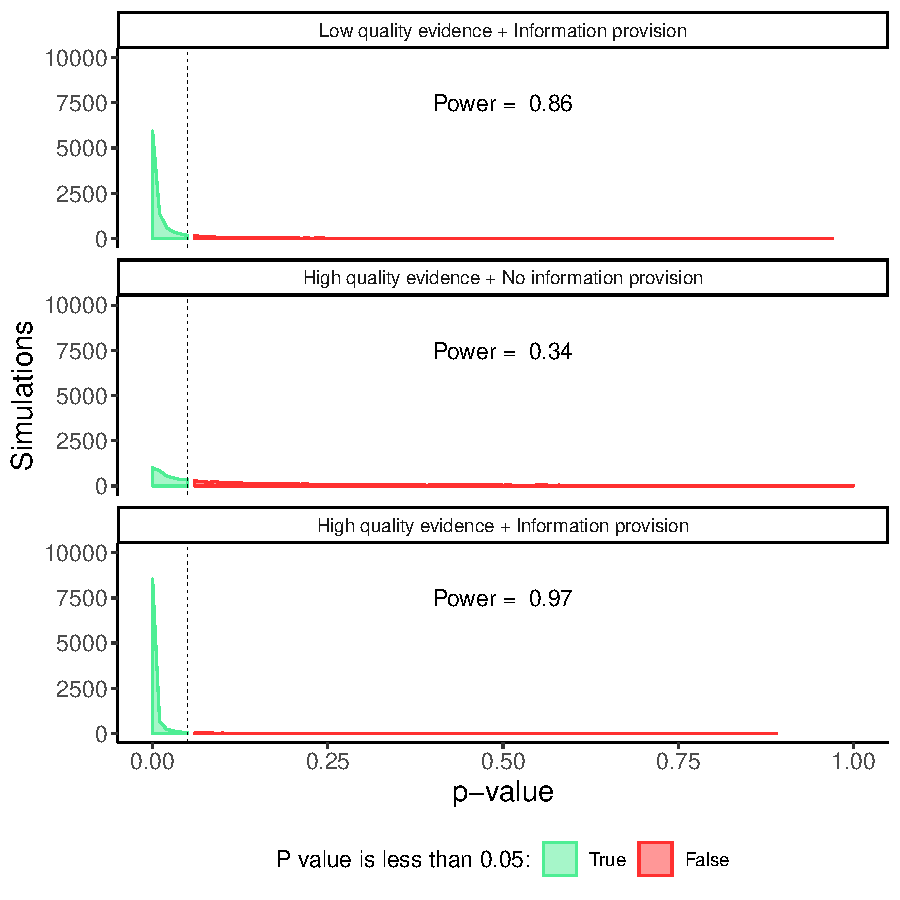
\includegraphics{../figs/power_fed.pdf}
\bigbreak
\caption{Power analysis: federal congress}
\label{fig: power_fed}
\end{figure}

We next conduct a power analysis using state legislatures. This theoretically could increase our possible sample size drastically, to roughly 5,000 respondents. However, we recognize that it would be logistically impractical for an organization to set up meetings with with such a large number of offices across such a wide geographical range. We therefore restrict ourself to a sample size of 1000, which could be achieved by sampling only from states in the Northeast United States, or from states where the organization has a local presence. Using the same assumptions of treatment effect sizes and variable that informed the power analysis in \autoref{fig: power_fed}, \autoref{fig: power_state} depicts the statistical power results from this increased sample size. The larger sample size results in statistical power of 0.99, 0.55, and 1 in treatment groups 2, 3, and 4, respectively.\footnote{Rounded to the nearest 100th decimal place.}

\begin{figure}[!htb]
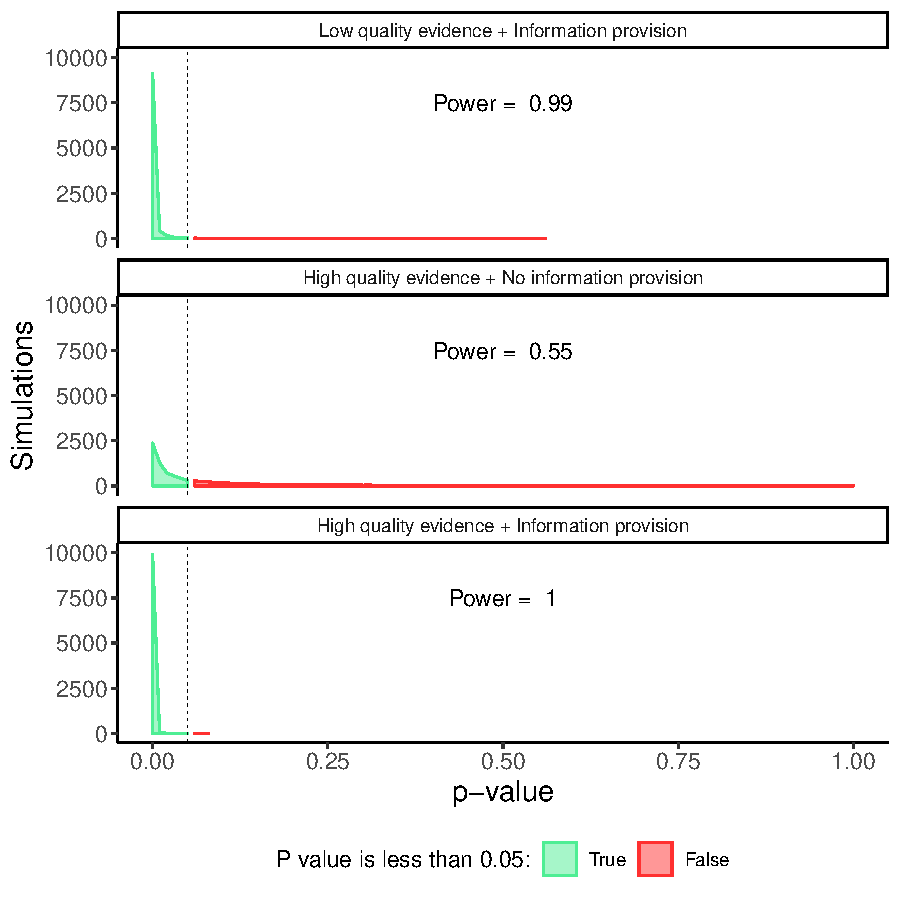
\includegraphics{../figs/power_state.pdf}
\bigbreak
\caption{Power analysis: state legislatures}
\label{fig: power_state}
\end{figure}



\section{Conclusion} \label{sec:Conclusion}

Our next steps on this project include finalization of some of the research design decisions that remain open (i.e. federal or state level subjects, partnership with an organization, and choice of the policy). We hope to finalize these details over the summer and to preregister a final Pre-Analysis-Plan with EGAP by the end of 2019. We would then conduct the experiment in 2020. We believe that this timeline would be ideal because of the political and electoral contexts expected in 2020. An election year increases the likelihood that parties will be seeking innovative policy ideas, and it is therefore possible that legislators will be particularly responsive to information on such policies. 



\clearpage
\pagebreak
\bibliography{bibliography}

\pagebreak

\appendix
\setcounter{table}{0}
\setcounter{figure}{0}
\renewcommand\thetable{\Alph{section}.\arabic{table}}
\renewcommand\thefigure{\Alph{section}.\arabic{figure}}
\section{Appendix} \label{Appendix}

\subsection{Department of Education evidence tiers} \label{sec: DoE}
\begin{figure}[!htb]
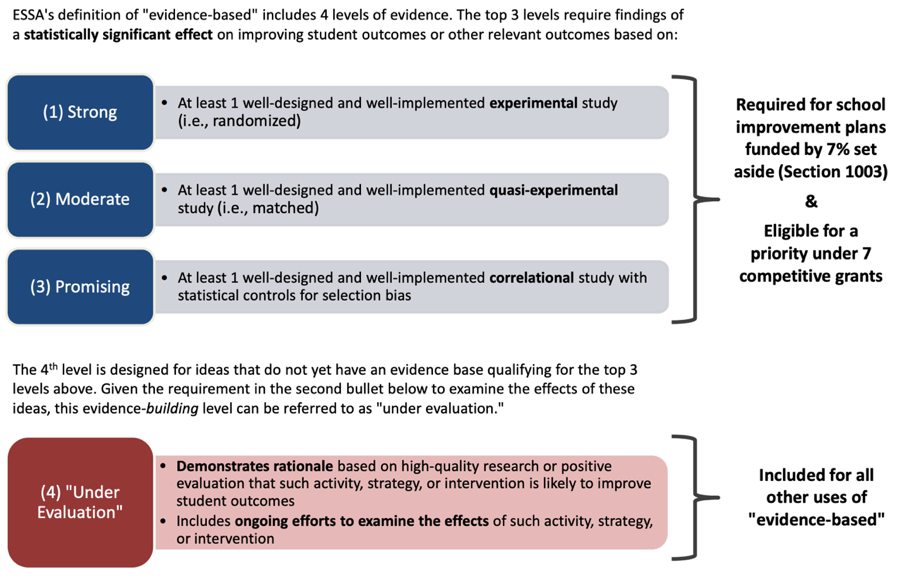
\includegraphics{../figs/doe_tiers.png}
\bigbreak
\caption{DoE's tiers of evidence}
\label{fig: doe_tiers}
\end{figure}

\end{document} 